\chapter{Modelo de maturidade}


	Um modelo de maturidade serve para avaliar a aptidão de uma organização afim de gerenciar seus projetos, são avaliados de acordo com as boas práticas de gerenciamento entre outros. Existem dois modelos de maturidade bastante utilizados pelas empresas brasileiras: o CMMI e o MPS.BR.

	O CMMI é um modelo de maturidade para desenvolvimento de software criado pelo SEI. Esse modelo é definido em áreas de processos que está vinculado às práticas relacionada satisfazendo um conjunto de objetivos oferecendo duas formas de abordagem diferentes para a melhoria de processos: modelo em estágio e modelo contínuo.
	
	O MPS é um programa para Melhoria de Processo do Software Brasileiro coordenado pela SOFTEX, com suporte do Ministério da Ciência e da Tecnologia, da FINEP e do BID. O MPS.BR é estruturado nos conceitos de maturidade dos processos para avaliação e melhoria da qualidade dos produtos de software e afins.

	\begin{figure}[!htpb]
			\centering
			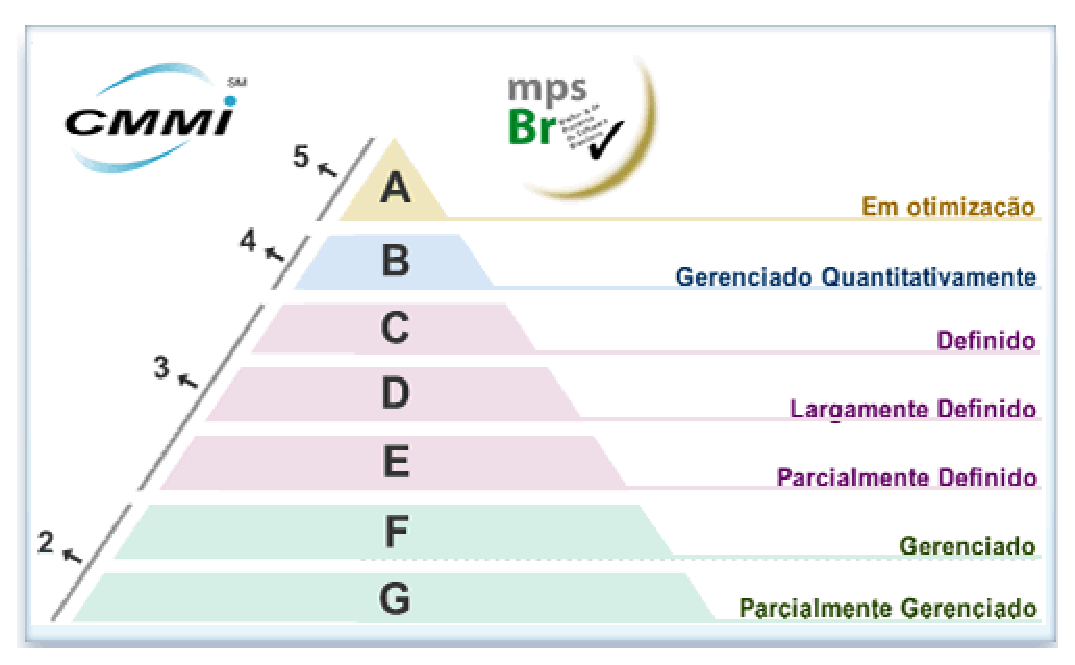
\includegraphics[scale=0.5]{figuras/maturidade/cmmi_mps}
			\caption{Níveis de maturidade}
	\end{figure}

	\section{}
